\section{Einleitung}\raggedbottom
\label{sec:Einleutung}
In dem ersten Kapitel der Arbeit wollen wir die Problematik und die Aufgabenstellung definieren. Dazu wird zunächst das Unternehmen Computer-Communications Networks GmbH (CoCoNet) vorgestellt. Nachdem die Arbeit dadurch in den Firmenkontext gebracht wird, wollen wir konkret die Fragestellung der Arbeit definieren und deren Aufbau beschreiben.
\subsection{Firmenprofil CoCoNet GmbH}
\label{sub:Firmenprofil CoCoNet GmbH}
Die Firma CoCoNet entwickelt digitale Banking-Lösungen für Unternehmen. In dieser Arbeit beschäftigen wir uns mit einem bestimmten CoCoNet Produkt, das \textit{Multiversa International Finance Portal} (IFP). Das IFP ist eine in Java implementierte Webanwendung, die alle gängigen Browser unterstützt. Nachdem sich ein User in das IFP eingeloggt hat, wird er zunächst zum Dashboard weitergeleitet. Das Dashboard ist die Startseite des \mbox{IFPs}, bestehend aus einer Navigationsleiste und Dashboardwidgets. Ein Widget ist eine Einheit, die auf dem Dashboard abgelegt werden kann und eine bestimmte Funktionalität hat. Von hier aus haben User die Möglichkeit durch das IFP zu navigieren, um z.B. eine Überweisung zu tätigen. \citep{CoCo20} \\
Für den weiteren Verlauf der Arbeit wollen wir nicht den kompletten Funktionsumfang des IFPs beleuchten, sondern uns auf das Dashboard mit seinen Widgets fokussieren.\\
Betrachten wir als Beispiel das \textit{Open Payments Widget} in Abbildung \ref{fig:open_payments}. 
\begin{figure}[htb]
\begin{center}
	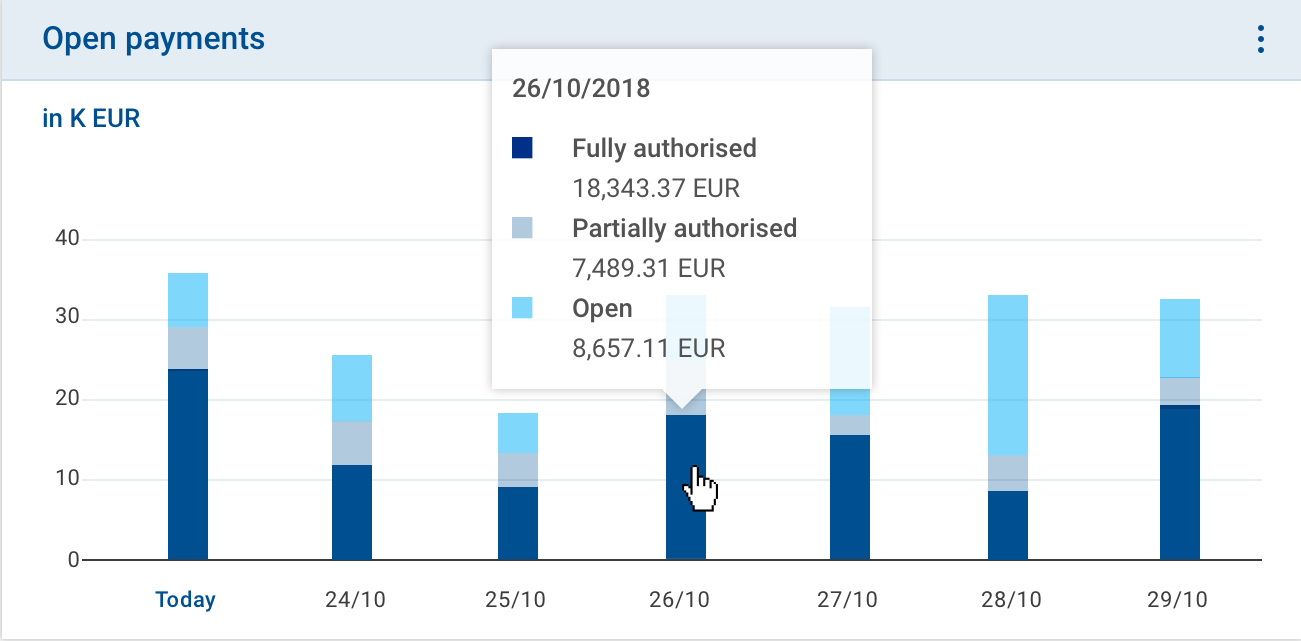
\includegraphics[width=400pt]{bilder/openPayments.png}
\end{center}
\caption{Open Payments Widget}
\label{fig:open_payments}
\end{figure}

Wie der Name schon vermuten lässt, zeigt das Widget Zahlungen an, die noch offen sind, also authorisiert werden müssen. Klickt man nun eine offene Zahlung an, wird man auf eine entsprechende Seite weitergeleitet, die mit den Zahlungsinformationen der selektierten Zahlung ausgefüllt ist.

\subsection{Ziel der Arbeit}
\label{sub:Problemstellung}
In dieser Arbeit geht es darum, das Userverhalten in Hinblick auf die Nutzung der Dash\-boardwidgets im IFP zu analysieren. Da der Begriff Userverhalten noch recht breit gefächert ist, sollen konkret die folgenden Fragen beantwortet werden:
\begin{enumerate}
	\item Wie oft werden Widgets in einem bestimmten Zeitraum benutzt? \label{intro:q1}\\
	\item Lässt sich ein bestimmter Workflow durch die Nutzung der Widgets erkennen?\\
\end{enumerate}
Diese Fragen wollen wir durch die Analyse von Logfiles beantworten.\\
Zunächst müssen wir aber definieren, was es bedeutet, ein Widgets zu benutzen. Da das Dashboard bzw. die Widgets das Erste sind, was man nach einem Login in das IFP sieht, könnte man meinen, dass das Vorhandensein auf dem Dashboard eine Nutzung schon einschließt. Betrachtet man z.B. das Widget in Abbildung \ref{fig:open_payments} stellt man fest, dass das Widget schon einiges an Informationen liefert. Allerdings kann man an dieser Stelle nur spekulieren, ob und in welchem Ausmaß der User diese Information wahrnimmt. Ein pures Vorhandensein des Widgets auf dem Dashboard ist als Nutzung nicht hinreichend. Erst ein Klick auf das Widget zählt als Nutzung.\\
Wenn nun ein Widget angeklickt wird, wird der Nutzer in der Regel auf eine neue Seite weitergeleitet, die durch das Widget z.B. schon vorgefiltert ist. Da diese Weiterleitung ein HTTP-Request an den Server ist, wird sie geloggt und kann in den Logfiles erkannt werden.\\
Also sind die Anforderungen an das zu entwickelnde System, dass die Nutzung eines Widgets erkannt wird und aus diesen Informationen Verhaltensmuster der User bzgl. der eben erwähnten Fragen erkannt werden. Außerdem soll das System nutzerfreundlich sein, damit es auch Menschen ohne besondere Vorkenntnisse benutzen können.\\
Ein weiteres Ziel der Arbeit ist eine kritische Einschätzung, inwiefern sich das entwickelte System für diese Art der Kundenanalyse eignet.\\

\subsection{Aufbau der Arbeit}
\label{sub:Aufbau der Arbeit}
Im folgenden Verlauf der Arbeit wird zunächst auf die theoretischen Grundlagen der Mustererkennung eingegangen. Dazu wird die Syntax der vorliegenden Logfile Einträge und anschließend die Phasen der Mustererkennung, die die Einträge durchlaufen, beschrieben. In dem darauf folgenden Kapitel wird dargelegt, wie die theoretischen Grundlagen technisch umgesetzt werden. Danach wird das entwickelte System getestet und die Ergebnisse diskutiert. Zum Schluss wird die Arbeit durch ein Fazit zusammengefasst und zukünftige Einsatzmöglichkeiten erörtert.

\clearpage



